
\chapter*{L'Optimisation du Code}
\section*{La division}

L'opération la plus lognue dans notre kernel est la division. A chaque exécution du kernel, celle-ci est éxécutée $n^2$ fois.

On inverse les boucles, ainsi on ne fait plus que $n$ divisions ; mais on doit faire en plus $n^2$ multiplications par appel du kernel.
\\Sur les processeurs Ivy Bridge, la multiplication est environ 3$\times$ plus rapide que la divsion. En considérant qu'une multiplication est faite en 1 cycle, on peut donc comparer.
Sans les boucles inversées,le traitement fait $n^2$ divsions, pour une durée de $3n^2$.
Avec les boucles inversées,le traitement fait $n$ divisions et $n^2$ multiplications, soit une durée de $3n+n^2$.
On compare $3n^2$ et $3n+n^2$:\\
\begin{figure}[ht!]
    \centering
    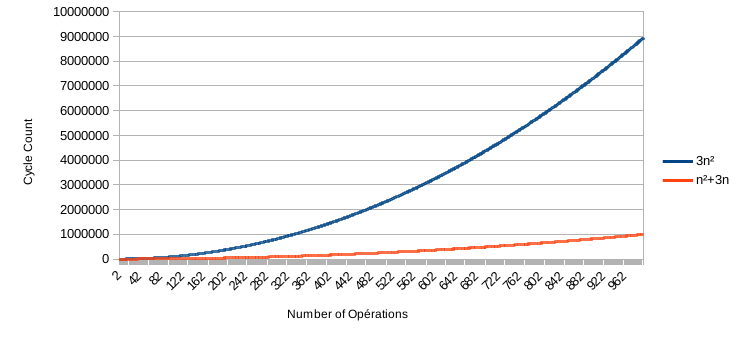
\includegraphics[width=100mm]{MEDIA/div_vs_mult_graph.png}
    \caption{Comparaison des temps de calcul des deux méthodes}
\end{figure}
Inverser les boucles est donc beaucoup plus rentable.
Speedup offert par cette optimisation:$\approx 3.11$.

\section*{Vectorisation}

La vectorisation est la possiblité de faire plus rapidement le même type d'opération a la suite, grâce a l'utilisation d'instructions et de registres particuliers.Le code peut être écrit de manière vectorisée, via l'utiliation d'intrinsics, ou bien cette optimisation peut-être faite par le compilateur.

Malheusement cela est impossible a cause de l'accès indirect; Nous cherchons donc un moyen de le retier.
\subsection*{L'accès indirect}
Cette méthode est faisable grâce a notre inversion de boucles.

Nous proposons d'ajouter une boucle au début du noyeau qui calculera les accés indrects avant que ceux-ci soient utilisés dans la bocule de calcul.
Ces données doivent être stockées entre le temps, la première idée serait d'ajouter un tableau supplémentaire a cet effet, mais il faudrait alors recalculer toutes les tailles de tableau pour le L1, L2, L3 et RAM (n valeurs supplémentaires a stocker).\\

Pour ne pas consommer plus de mémoire, nous avons donc décidé de stocker ces valeurs sur la dernière ligne du tableau résultat.
Lors du calcul de la dernière ligne, l'indice indirect est donc lu pour la dernière fois juste avant d'être remplacé par le résultat. 

\subsection*{Vectorisé!}
Avant de supprimer l'accès indirect via la 1ère boucle, il était impossible pour les compilateurs de vectoriser le code.

Maintenant nous avons un code vectorisé a:
    \begin{itemize}
    \item{$66\%$ avec gcc}
    \item{$75\%$ avec icc}
    \end{itemize}

    Le code est vectorisé avec des instructions AVX, qui utilisent des registres de 256 bits. On peut donc stocker 8 floats/int32\_t par registre AVX.
    Il n'est pas vraiment possible de donner le speedup individuel de cette optimisation, car elle dépend de l'inversion des boucles.
Speedup avec ces deux optimisations :$\approx 7.11$
\section*{Tiling}
Nous avons également envisagé de faire du tiling. Le tiling est une méthode consistant a découper le traitement de la matrice en un ensemble de sous-traitements sur des sous-ensembles de cette matrice..Ces matrices étant plus petites, elle peuvent être chargées dans des niveaux de cahche plus rapides, et donc accélérer le traitement.
Malheursement, nous nous sommes rapidement rendus compte que cette méthode n'était pas adaptée a notre traitement.
En effet le tiling a un intérêt seulment quand une même partie de matrice est réutilisée plusieurs fois, ce qui n'est pas notre cas.
De plus, cela nuirait a notre optimisation sur la division, si par exemple on découpe notre matrice en 100 blocs de même taille, il nous faudra faire $10\times n $ divisions.

Nous n'avons donc pas appliqué cette methode.

\section*{Optimisations Compilateur}

Nous avons également utilisé un flag de compilation supplémentaire, afin d'aller toujours plus vite.
Ce flag s'écrit --march=native pour gcc et -xHost pour icc. Il indique au compilateur que le code est destiné exculsivement au processeur utilisé pour la compilation, et permet donc une optimisation plus poussée.\\
\begin{itemize}
    \item{Speedup pour gcc (Avec les autres opti):$\approx 8.97$}
    \item{Speedup pour icc (Avec les autres opti):$\approx 11.30$}\\
\end{itemize}



